\documentclass[10pt,twocolumn,letterpaper]{article}

\usepackage{cvpr}
\usepackage{times}
\usepackage{epsfig}
\usepackage{graphicx}
\usepackage{amsmath}
\usepackage{amssymb}
\usepackage{subfigure}
\usepackage{upgreek}
\usepackage{multirow}
\usepackage{color}
\DeclareMathOperator*{\argmin}{arg\,min}


% Include other packages here, before hyperref.

% If you comment hyperref and then uncomment it, you should delete
% egpaper.aux before re-running latex.  (Or just hit 'q' on the first latex
% run, let it finish, and you should be clear).
\usepackage[pagebackref=true,breaklinks=true,letterpaper=true,colorlinks,bookmarks=false]{hyperref}

% \cvprfinalcopy % *** Uncomment this line for the final submission

\def\cvprPaperID{****} % *** Enter the CVPR Paper ID here
\def\httilde{\mbox{\tt\raisebox{-.5ex}{\symbol{126}}}}

% Pages are numbered in submission mode, and unnumbered in camera-ready
\ifcvprfinal\pagestyle{empty}\fi


\begin{document}

%%%%%%%%% TITLE
\title{External Patch Group Prior Guided Internal Orthogonal Dictionary Learning for Real Image Denoising}

\author{First Author\\
Institution1\\
Institution1 address\\
{\tt\small firstauthor@i1.org}
% For a paper whose authors are all at the same institution,
% omit the following lines up until the closing ``}''.
% Additional authors and addresses can be added with ``\and'',
% just like the second author.
% To save space, use either the email address or home page, not both
\and
Second Author\\
Institution2\\
First line of institution2 address\\
{\tt\small secondauthor@i2.org}
}

\maketitle 


%%%%%%%%% ABSTRACT
\begin{abstract}
For image denoising problem, the external and internal priors are playing key roles in many different methdos. External priors learn from external images to restore noisy images while internal ones exploit priors of given images for denoising. The external priors are more generative and efficient on recovering structures existing in most images while the internal priors are more adaptive on recovering detials existed in given noisy images. In this paper, we propose to employ the external patch group prior of images to guide the clustering of internal patch groups, and develop an external dictionary guided internal orthogonal dictionary learning algorithm for real image denoising. The internal orthogonal dictionary learning process has closed-form solutions and hence very efficient for online denoising. The experiments on standard datasets demonstrate that, that the proposed method achieves better performance than other state-of-the-art methods on real image denoising. 
\end{abstract}
%Though these methods are very effective in Gaussian noise removal, the noise in real images are signal dependent and more complex than Gaussian noise. Therefore, only exploiting the external or internal priors are not enough for real image denoising.

%%%%%%%%% BODY TEXT
\section{Introduction} 
Most vision systems, such as medical imaging and surveillance, need accurate feature extraction from high-quality images. The camera sensors and outdoor low light conditions will unavoidly bring noise to the captured images. The impact is that the image details will be lost or hardly visible. As a result, image denoising is an essential procedure for the reliability of these vision systems. In the research ara, image denoising is also an ideal platform for testing natural image models and provides high-quality images for other conputer vision tasks such as image registration, segmentation, and pattern recognition, etc. 

For several decades, there emerge numerous image denoising methods \cite{nlm,foe,ksvd,bm3d,lssc,epll,mlp,wnnm,csf,pgpd,chen2015learning}, and all of them focus mainly on dealing with additive white Gaussian noise (AWGN). In real world, the cameras will undertake high ISO settings for high-speed shots on actions, long exposure for low light on night shots, etc. Under these situations, the noise is generated in a complex form and also been changed during the in-camera imaging pipeline \cite{NewInCamera,crosschannel2016}. Therefore, the noise in real images are much more complex than Gaussian \cite{crosschannel2016,healey1994radiometric}. It depends on camera series, brands, as well as the settings (ISO, shutter speed, and aperture, etc). The models designed for AWGN would become much less effective on real noisy images. 

In the last decade, the methods of \cite{fullyblind,rabie2005robust,Liu2008,almapg,noiseclinic,Zhu_2016_CVPR,crosschannel2016} are developed to deal with real noisy images. Almost all these methods employ a two-stage framework: estimating the parameters of the assumed noise model (usually Gaussian) and performing denoising with the help of the noise modeling and estimation in the first stage. However, the Gaussian assumption is inflexible in describing the complex noise on real noisy images \cite{Liu2008}. Although the mixture of Gaussians (MoG) model is possible to approximate any noise distribution \cite{Bishop}, estimating its parameters is time consuming via nonparametric Bayesian techniques \cite{Zhu_2016_CVPR}. To evaluate the performanec of these methods on dealing with complex real noise, we apply these methods, with corresponding default parameters, on a real noisy image provided in \cite{crosschannel2016}. The testing image is captured by a Nikon D800 camera when ISO is 3200. The "ground truth" image is also provided with which we can calculate objective measurements such as PSNR and SSIM \cite{ssim}. The denoised images are listed in Figure \ref{fig1}, from which we can see that these methods either remove the noise or oversmooth the complex details in real noisy image. 
\begin{figure*}\label{fig1}
\centering
\subfigure{
\begin{minipage}[t]{0.195\textwidth}
\centering
\raisebox{-0.15cm}{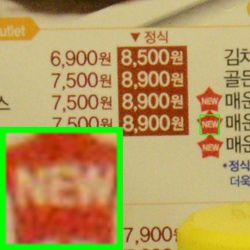
\includegraphics[width=1\textwidth]{images/resize_br_Noisy_CC_Noisy_Nikon_D800_ISO_3200_A3_66.png}}
{\footnotesize (a) Noisy Image \\ (33.30dB/0.8921) }
\end{minipage}
\begin{minipage}[t]{0.195\textwidth}
\centering
\raisebox{-0.15cm}{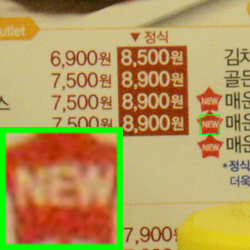
\includegraphics[width=1\textwidth]{images/resize_br_CBM3D_CC_Noisy_Nikon_D800_ISO_3200_A3_66.png}}
{\footnotesize (b) CBM3D \cite{cbm3d} \\ (33.33dB/0.8935)  }
\end{minipage}
\begin{minipage}[t]{0.195\textwidth}
\centering
\raisebox{-0.15cm}{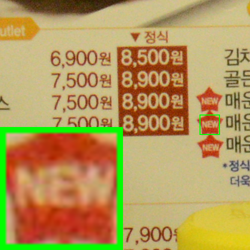
\includegraphics[width=1\textwidth]{images/resize_br_WNNM_CC_Noisy_Nikon_D800_ISO_3200_A3_66.png}}
{\footnotesize (c) WNNM \cite{wnnm}\\ (33.30dB/0.8922)  }
\end{minipage}
\begin{minipage}[t]{0.195\textwidth}
\centering
\raisebox{-0.15cm}{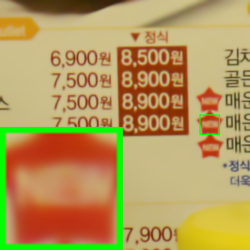
\includegraphics[width=1\textwidth]{images/resize_br_MLP_CC_Noisy_Nikon_D800_ISO_3200_A3_66.png}}
{\footnotesize (d) MLP \cite{mlp}\\ (34.22dB/0.9603) }
\end{minipage}
\begin{minipage}[t]{0.195\textwidth}
\centering
\raisebox{-0.15cm}{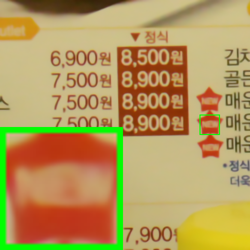
\includegraphics[width=1\textwidth]{images/resize_br_CSF_CC_Noisy_Nikon_D800_ISO_3200_A3_66.png}}
{\footnotesize (e) CSF \cite{csf}\\ (35.39dB/0.9677) }
\end{minipage}
}\vspace{-3mm}
\subfigure{
\begin{minipage}[t]{0.195\textwidth}
\centering
\raisebox{-0.15cm}{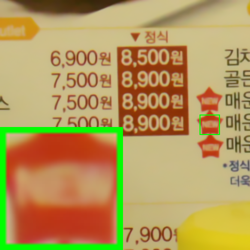
\includegraphics[width=1\textwidth]{images/resize_br_TRD_CC_Noisy_Nikon_D800_ISO_3200_A3_66.png}}
{\footnotesize (f) TRD \cite{chen2015learning} \\ (35.97dB/0.9705)   }
\end{minipage}
\begin{minipage}[t]{0.195\textwidth}
\centering
\raisebox{-0.15cm}{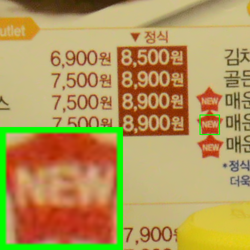
\includegraphics[width=1\textwidth]{images/resize_br_NC_CC_Noisy_Nikon_D800_ISO_3200_A3_66.png}}
{\footnotesize (g) Noise Clinic \cite{noiseclinic} \\ (35.33dB/0.9520)  }
\end{minipage}
\begin{minipage}[t]{0.195\textwidth}
\centering
\raisebox{-0.15cm}{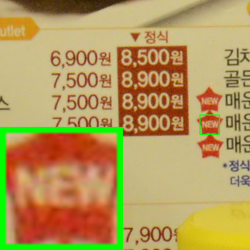
\includegraphics[width=1\textwidth]{images/resize_br_NI_CC_Noisy_Nikon_D800_ISO_3200_A3_66.png}}
{\footnotesize (h) Neat Image \cite{neatimage}\\ (34.39dB/0.9314)  }
\end{minipage}
\begin{minipage}[t]{0.195\textwidth}
\centering
\raisebox{-0.15cm}{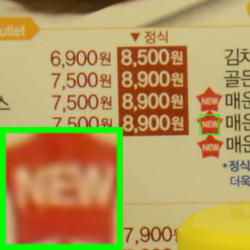
\includegraphics[width=1\textwidth]{images/resize_br_Guided_CC_Noisy_Nikon_D800_ISO_3200_A3_66.png}}
{\footnotesize (i) Ours \\ (\textbf{37.28}dB/\textbf{0.9729})  }
\end{minipage}
\begin{minipage}[t]{0.195\textwidth}
\centering
\raisebox{-0.15cm}{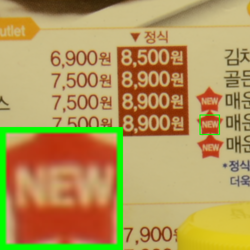
\includegraphics[width=1\textwidth]{images/resize_br_Mean_CC_Noisy_Nikon_D800_ISO_3200_A3_66.png}}
{\footnotesize (j) Mean Image }
\end{minipage}
}\vspace{-1mm}
\caption{Denoised images of the real noisy image "Nikon D800 ISO 3200 A3" from \cite{crosschannel2016} by different methods. The images are better viewed by zooming in on screen.} \vspace{-4mm}
\end{figure*}

The above mentioned methods can be categorized into external methods which learn priors from external images to recover noisy images, and internal ones which exploit priors of given images for denoising. The external priors in natural images are free of the high correlation between noise and siganls in real noisy images, while the internal prior is adaptive to the image and can recover better the latent clean image. Combining the priors of external clean images and adaptivety of internal testing images can naturally improve the performance of denoising methods, especially on real noisy images. Based on these observations, in this paper, we propose to employ the external patch group prior \cite{pgpd} of natural clean images to guide the clustering of internal patch groups in given noisy image, and develop an external prior guided internal orthogonal dictionary learning (DL) algorithm for real image denoising. The internal orthogonal DL process includes two alternating stages: updating sparse coefficients and updating orthogonal dictionary. Both of the two stages have closed-form solutions. Hence, our internal DL process is very efficient for online internal denoising. Through comprehensive experiments on real noisy images captured by different cameras and settings, we demonstrate that the proposed method achieves better performance on real image denoising

\subsection{Our Contributions}
The contributions of this paper are summarized as follows:
\begin{itemize}
\item We propose a noval dictionary learning method which employ the external prior guided the internal orthogonal dictionary learning for real image denoising. Both the external prior and internal prior are performed on patch groups instead of patches.
\item The internal orthogonal dictionary learning are alternating iterative solved with closed-form solutions. The learned orthogonal dictionary are very efficient in both learning and denoising stages. 
\item We achieve much better performance on the real image denoising problem than other competing methods in terms of visual quality, PSNR, and SSIM.
\end{itemize}

The rest of this paper will be summerized as follows: in Section 2, we will introduce the related work; in Section 3, we will introduce the proposed external prior guided internal orthogonal dictionary learning algorithm for real image denoising; in Section 4, we will demonstrate the extensive experiments on two standard dataset; we will conclude our paper and give our future work in Section 5.

\section{Related Work}
\subsection{Patch Group Prior of Natural Images}
The Patch Group (PG) prior \cite{pgpd} is proposed to directly model the non-local self similar (NSS) property of natural images. The NSS property is commonly used in image restoration tasks \cite{nlm,bm3d,lssc,wnnm,pgpd}. The PG prior largely reduces the space of images to be modeled when compared to the patch prior \cite{epll}. In \cite{pgpd}, only the PGs of clean natural images is utilized, while the PGs of noisy input images are ignored. In this paper, we make use of PGs both from external clean images and internal given real noisy image for better denoising performance.

%In fact, we use the external Pacth Group prior to guide the structural clustering of internal patch groups in real noisy images. For each cluster of PGs, we propose to use PCA for subspace learning. The eigenvectors are the basis of this subspace and hence can be used as an orthonormal dictionary. The eigenvalues reflect the information describing the noise levels and hence can be used as parameters for image denoising. Noted that the dictionary and parameters are obtained via a fully unsupervised way by subspace learning. Therefore, our model is highly adaptive to the noisy input images.

\subsection{Internal v.s. External Dictionary Learning}
Learning dictionaries to represent images has been successfully used in image modeling \cite{ksvd,ksvdtsp,epll,ple,ncsr,pgpd}.There are mainly two categories of DL methods: 1) External DL methods pre-learned dictionary from a set of clean image patches, and the learned dictionaries are used to encode the noisy image patches for denoising \cite{ksvdtsp,epll,pgpd}. 2) Internal DL methods directly learned dictionary from the patches of given noisy image, and the image denoising is simultaneously done with the DL process \cite{ksvd,ple,ncsr}. The external DL methods is not adaptive to the noisy image, while the internal DL methods is adaptive to the degraded images but it ignores the information hidden in clean images. In this paper, our goal is to employ the external dictionary to guide the learning of internal orthogonal dictionary.

\subsection{Real Image Denoising}
In the last decade, there are many methods \cite{fullyblind,rabie2005robust,Liu2008,almapg,noiseclinic,Zhu_2016_CVPR,crosschannel2016} proposed for real image denoising problem. In the seminar work of BLS-GSM \cite{blsgsm} for real image denoising, Portilla et al. proposed to use scale mixture of Gaussian in overcomplete oriented pyramids to estimate the latent clean images. In \cite{fullyblind}, Portilla proposed to use a correlated Gaussian model for noise estimation of each wavelet subband. The work of Rabie \cite{rabie2005robust} modeled the noisy pixels as outliers which are removed via Lorentzian robust estimator \cite{huber2011robust}. Liu et al. \cite{Liu2008} proposed to use 'noise level function' (NLF) to estimate the noise and then use Gaussian conditional random field to obtain the latent clean image. Gong et al. \cite{almapg} models the noise by mixed $\ell_{1}$ and $\ell_{2}$ norms and remove the noise by sparsity prior in the wavelet transform domain. Later, Lebrun el al. proposed a multiscale denoising algorithm called 'Noise Clinic' \cite{noiseclinic}. This method generalizes the NL-Bayes model \cite{nlbayes} to deal with blind noise and achieves state-of-the-art performance. Recently, Zhu et al. proposed a Bayesian model \cite{Zhu_2016_CVPR} which approximates and remove the noise via Low-Rank Mixture of Gaussians (LR-MoG). The commercial software Neat Image \cite{neatimage} first estimates the parameters of noise via a large flat area and then filters the noise accordingly.

\section{External Patch Group Prior Guided Internal Orthogonal Dictionary Learning}
In this section, we formulate the framework of external patch group (PG) prior guided internal orthogonal dictionary learning. We first introduce the patch PG leaning on clean natural RGB images. Then we propose to exploy the external PG prior to guide the internal clustering and orthogonal dictionary learning (DL). The orthogonal DL has alternative closed-form solutions in term of updating sparse coefficients and dictionary. Finally, we discuss the advantages of our proposed external PG prior guided internal orthogonal dictionary learning algorithm.

\subsection{External Patch Group Prior Learning}
Natural images often demonstrate repepitive local patterns, this nonlocal self-similarity (NSS) property is a key successful factor for many image denoising methods \cite{nlm,bm3d,lssc,ncsr,wnnm,pgpd}. In this section, we formulate the Patch Group prior learned on natural color images. Similar to \cite{pgpd}, the patch group (PG) is defined as a group of similar patches to the local patch. The patch group mean is destracted, and hence different groups patches can share similar PGs. In this way, the space natural image patches to be modeled is largely reduced. In this work, each local patch extracted from RGB images is of size $p\times p \times 3$. Then we search the $M$ most similar patches $\{\mathbf{x}_{m}\}_{m=1}^{M}$ around each local patch through Euclidean distance, in a local window of size $W\times W$. The $\mathbf{x}_{m}\in \mathbb{R}^{3p^{2}\times1}$ is a patch vector formed by combining the 3 patch vectors (of size $p^{2}\times 1$) in R, G, B channels. The mean vector of this PG is $\boldsymbol{\upmu}=\frac{1}{M}\sum_{m=1}^{M}\mathbf{x}_{m}$, and the group mean subtracted PG is defined as $\mathbf{\overline{X}}\triangleq \{\mathbf{\overline{x}}_{m}=\mathbf{x}_{m}-\boldsymbol{\upmu}\}, m=1,...,M$. Assume we have extracted $N$ PGs from a set of external natural images, and the $n$-th PG is defined as $\mathbf{\overline{X}}_{n}\triangleq \{\mathbf{\overline{x}}_{n,m}\}_{m=1}^{M}, n=1,...,N$. We employ the Gaussian Mixture Model (GMM) to learn the external patch group based NSS prior. In this model, the likelihood of the $n$-th PG $\{\mathbf{\overline{X}}_{n}\}$ can be calculated as
\vspace{-2mm}
\begin{equation}\label{equ1}\vspace{-2mm}
P(\mathbf{\overline{X}}_{n})  = \sum\nolimits_{k=1}^{K}\pi_{k}\prod\nolimits_{m=1}^{M}\mathcal{N}(\mathbf{\overline{x}}_{n,m}|\boldsymbol{\upmu}_{k},\mathbf{\Sigma}_{k}),
\end{equation}
where $K$ is the number of Gaussians and the $k$-th Gaussian is $\{\mathcal{N}(\boldsymbol{\upmu}_{k},\mathbf{\Sigma}_{k})\}$. By assuming that all the PGs are independently sampled, the overall objective log-likelihood function is
\vspace{-2mm}
\begin{equation}\label{equ2}\vspace{-2mm}
\begin{split}
\ln\mathcal{L}=\sum_{n=1}^{N} \ln(\sum_{k=1}^{K}\pi_{k}\prod_{m=1}^{M}\mathcal{N}(\mathbf{\overline{x}}_{n,m}|\boldsymbol{\upmu}_{k},\mathbf{\Sigma}_{k})).
\end{split}
\end{equation} 
We maximize the above objective function for PG-GMM learning and  finally obtain the GMM model with learned parameters including mixture weights $\{\pi_{k}\}_{k=1}^{K}$, mean vectors $\{\boldsymbol{\upmu}_{k}=\mathbf{0}\}_{k=1}^{K}$, and covariance matrices $\{\mathbf{\Sigma}_{k}\}_{k=1}^{K}$. Noted that the mean vector of each cluster is natural zeros, i.e., $\boldsymbol{\upmu}_{k}=\mathbf{0}$.

\subsection{External Prior Guided Internal Orthogonal Dictionary Learning}
Given a rael noisy image, we extract noisy PGs from it and save the mean vectors of each PG for recovering. The mean substracted PG is defined as $\mathbf{\overline{Y}}$. To project this PG into a most adaptive subspace, we select the most suitable Gaussian component to it from the PG-GMM trained in previous section. The selection can be done by checking the posterior probability that $\mathbf{\overline{Y}}$ belongs to the $k$th Gaussian component:
\begin{equation}\label{equ3}
P(k|\mathbf{\overline{Y}})=\frac{\prod_{m=1}^{M}\mathcal{N}(\mathbf{\overline{y}}_{m}|\mathbf{0},\mathbf{\Sigma}_{k})}{\sum_{l=1}^{K}\prod_{m=1}^{M}\mathcal{N}(\mathbf{\overline{y}}_{m}|\mathbf{0},\mathbf{\Sigma}_{l})}.
\end{equation}
Since the noise on real images are mostly small when compared to the signals, the covariance matrix of the $k$th component is still $\mathbf{\Sigma}_{k}$. Finally, the component with the maximum A-posteriori (MAP) probability $\ln P(k|\mathbf{\overline{Y}})$ is selected as the most suitable subspace for $\mathbf{\overline{Y}}$.

Though each PG has been projected into its most suitable subspace, the pre-learned subspace is still too general to represent the noisy PG extracted from the real noisy image. That is, the noisy PGs projected into one cluster can still constisted a subspace which is of lower dimensions than the subspace pre-learned from the external PGs. This can be demonstrated by compare the distribution of external PGs and internal PGs in the same clusters. We randomly select one cluster, and collect the celan PGs extracted from external dataset (Kodak 24 images) and the niosy PGs from the testing image. Since the original PGs are of $3p^{2}$ dimensions, we apply PCA to project the PGs into 2 dimensions for better visualization. The results is shown in Figure \ref{fig}, from which we can see clearly that the projected PGs are mainly in a smaller region of the external PGs, which proves that the internal PGs are only consisted a subspace in a lower dimension than the PGs collected from external subspace. To better and adaptively charactering the internal PGs from the testing image, we need learn a more specific dictionary for noisy PGs assigned into each cluster. For notation simplicity, we ignore the index of subspace $k$. The internal PGs $\mathbf{Y}$ form a subspace which can be obtained by singular value decomposition (SVD),
\begin{equation}\label{equ4}
\begin{split}
&\min_{\mathbf{D}_{i}\in \mathbb{R}^{3p^2\times r},\textbf{A}\in\mathbb{R}^{3p^2\times MN}}
\|\mathbf{Y}-[\mathbf{D}_{e}\ \mathbf{D}_{i}]\mathbf{A}\|_{F}^{2}+\lambda\|\mathbf{A}\|_{1}
\\
&
\text{s.t.}
\quad
\mathbf{D}_{i}^{T}\mathbf{D}_{i} = \mathbf{I}_{r},\ \mathbf{D}_{e}^{T}\mathbf{D}_{i} = \mathbf{0},
\end{split}
\end{equation}
The singular vectors capture the statistical structures of NSS variations in natural images, while the singular values in $\mathbf{S}$ represent the significance of these singular vectors. Fig.\ 4 shows the singular vectors for one Gaussian component.

\subsection{Optimization with Closed-form Solution}
Similar to the K-SVD \cite{ksvd}, we employ an alternating iterative framework to solve the optimization problem \ref{equ4}. In fact, we initialize the orthogonal dictionary as $\mathbf{D}^{(0)}$ and for $t=0, 1, ..., T-1$, alternatively do

\textbf{Updating Sparse Coefficients}: given the initialization orthogonal dictioanry $\textbf{D}_{i}^{(t)}$, the sparce coefficients 
$\textbf{A}^{(t)}$ are obtained via solving
\begin{equation}\label{equ5}
\textbf{A}^{(t)}:=\argmin_{\textbf{A}\in\mathbb{R}^{3p^2\times MN}}
\|\mathbf{Y}-[\mathbf{D}_{e}\ \mathbf{D}_{i}^{(t)}]\mathbf{A}\|_{F}^{2}+\lambda\|\mathbf{A}\|_{1}.
\end{equation}
This problem has closed-form solution by $\mathbf{A}^{*}=T_{\lambda}(\mathbf{\hat{D}}^{T}\mathbf{Y})$, 
where $T_{\lambda}(\mathbf{A}) = \text{sgn}(\mathbf{A})\odot\max(\mathbf{A},\lambda)$ is a soft-thresholding function.

\textbf{Updating Orthogonal Dictionary}: given the sparse coefficients $\textbf{A}^{(0)}$, the sparce coefficients 
$\textbf{A}^{(t)}$ are obtained via solving
\begin{equation}\label{equ6} 
\begin{split}
\textbf{D}_{i}^{(t+1)}:=
&
\argmin_{\textbf{D}_{i}\in\mathbb{R}^{3p^2\times r}}
\|\mathbf{Y}-[\mathbf{D}_{e}\ \mathbf{D}_{i}]\mathbf{A}^{(t)}\|_{F}^{2}
\\
&
\text{s.t.}
\quad
\mathbf{D}_{i}^{T}\mathbf{D}_{i} = \mathbf{I}_{r},\ \mathbf{D}_{e}^{T}\mathbf{D}_{i} = \mathbf{0},
\end{split}
\end{equation}
Dividing the sparse coefficients $\mathbf{A}=[\mathbf{A}_{e}^{T}\ \mathbf{A}_{i}^{T}]^{T}$, where $\mathbf{A}_{e}$ and $\mathbf{A}_{i}$ denote the coefficients over external and internal dictionary $\mathbf{D}_{e}$ and $\mathbf{D}_{i}$. According to the Proposition 2.2 in \cite{bao2013fast}, the problem (\ref{equ6}) 
%\begin{equation}
%\begin{split}
%\min_{\textbf{D}_{i}\in\mathbb{R}^{3p^2\times r}}
%&\|\mathbf{Y}-\mathbf{D}_{e}\mathbf{A}_{e}+\mathbf{D}_{i}\mathbf{A}_{i}\|_{F}^{2}
%\\
%&
%\text{s.t.}
%\quad
%\mathbf{D}_{i}^{T}\mathbf{D}_{i} = \mathbf{I}_{r},\ \mathbf{D}_{e}^{T}\mathbf{D}_{i} = \mathbf{0},
%\end{split}
%\end{equation}
has a closed-form solution $\mathbf{D}_{i}^{*}=\mathbf{U}\mathbf{V}^{T}$, where $\mathbf{U}$ and $\mathbf{V}$ are
the orthogonal matrices obtained by the following SVD
\begin{equation}\label{equ7}
(\mathbf{I}-\mathbf{D}_{e}\mathbf{D}_{e}^{T})\mathbf{Y}\mathbf{A}_{i}^{T}
=
\mathbf{U}\Sigma\mathbf{V}^{T}
\end{equation}
With these solutions, the final obtained dictionary $\mathbf{D} = [\mathbf{D}_{e}\ \mathbf{D}_{i}]$ are orthogonal ictionary. This can be proved by the following equation
\begin{equation}\label{equ8}
\mathbf{D}^{T}\mathbf{D} = 
\left(\begin{array}{c}
\mathbf{D}_{e}^{T}
\\
\mathbf{D}_{i}^{T}
\end{array}\right)
(\mathbf{D}_{e}\ \mathbf{D}_{i})
=
\left(\begin{array}{cc}
\mathbf{D}_{e}^{T}\mathbf{D}_{e}\ \mathbf{D}_{e}^{T}\mathbf{D}_{i}
\\
\mathbf{D}_{i}^{T}\mathbf{D}_{e}\ \mathbf{D}_{i}^{T}\mathbf{D}_{i}
\end{array}\right)
=
\mathbf{I}
\end{equation}

\subsection{Discussion on External Prior and Internal Orthogonal Dictionary Learning}
Until now, we have divided the noisy PGs into multiple internal subspaces. Here we take a deep analysis on how the external NSS prior guide the subspace learning of internal PGs. The help are at least threefold. Firstly, through MAP in (\ref{equ3}), the external prior guides the noisy PGs to be clustered into the correct subspaces. If we cluster the noisy PGs in an automatical way, the subspaces we learned will be highly degraded by the signal dependent noise. Secondly, the guidance of external prior for internal clustering is more efficient than directly clustering the internal noisy PGs. It only needs to calculate the MAP probability via the equation (\ref{equ3}) while the internal clustering via GMM is time-consuming on EM algorithm \cite{em}. Thirdly, due to the correct guidance of external prior, the structual decomposition via SVD of each subspace is more adaptive. This will bring better denoising performance than the methods only using the external information. The \emph{mutual incoherence} $\mu(\mathbf{U})$ \cite{donoho2003optimally}, which is difined as
\begin{equation}\label{equ9}
\mu(\mathbf{U})=\max_{i~=j}\frac{|\mathbf{d}_{i}^{T}\mathbf{d}_{j}|}{\|\mathbf{d}_{i}\|_{2}\|\mathbf{d}_{j}\|_{2}}
\end{equation},
is a measure of quality of dictionary.

The Internal PGs are in fact lying in the subspaces of external PG Spaces. To defend this argument, we compare the distribution of external PGs extracted from clean natural images and real noisy images. For better illumination, we randomly selected a cluster and project the original clean PGs $\mathbf{X}$ onto a 2-D plane. This could be done via $\mathbf{Xp}=\mathbf{U(:.1:2)}^{T}\mathbf{X}$, where $\mathbf{U}$ is the singular vector matrix of that cluster. The noisy PGs $\mathbf{Y}$ assigned in this cluster is also projected into 2-D via $\mathbf{Yp}=\mathbf{U(:.1:2)}^{T}\mathbf{Y}$. The Figure \ref{} reflects the distribution on the 2-D plane of the projected clean PGs from external natural images and the projected noisy PGs from internal image. We can see that the internal noisy PGs are indeed lying in a subspace of the external PGs. Hence, if we directly use the external prior learned from clean PGs, the learned subspaces would be too generative to be suitable for the testing data. 

Through SVD, the PGs in each internal subspace can be divided into singular vectors and singular values. The singular vectors are the basis of the corresponding subspace while the singular values reflect the importance of these basis. The basis can be used as dictionary to code the noisy PGs. And the sigular values are adaptive parameters for internal noisy PGs. We can compare the singular values of one internal subspace and the corresponding space of external PGs. The result is shown in Figure \ref{}. From which we can see that the noisy subspace often have higher values than external space consisted of clean PGs. This gap is clearly made of the noise and can be used for image denoising in a natural way.


\section{The Denoising Algorithm}
\subsection{Fast Patch Group Searching by Integral Image}
The searching of patch groups in images is inefficient if we search non-local similar patches to each local patch. To speed up the searching process and make our proposed method faster, we employ the technique of 'Summed Area Table' \cite{sat} for efficient PG searching. The SAT permits to evaluate the sum of pixel values in rectangular regions of the image with four operations, regardless of the region size. That is to say, we do not need do distance measure for each patch. It was first proposed under the name of summed area table\cite{viola2004robust}

\subsection{Prior Weights for Sparse Coding}
To remove the real noise, we employ the sparse coding framework. And in order to be adaptive to the input image, we employ the internal learned $\mathbf{U}$ of each cluster as an adaptive dictioanry to represent the structural variations of the PGs in that cluster. Since the $\mathbf{U}$ is orthonormal, its \emph{mutual incoherence} is naturally $0$ and therefore better than other redundant dictionaries. 

\begin{equation}\label{equ10}
\min\nolimits_{\boldsymbol{\upalpha}}\|\mathbf{\overline{y}}_{m}-\mathbf{U}\boldsymbol{\upalpha}\|_{2}^{2}+\sum_{i=1}^{3p^{2}}\lambda_{i}|\boldsymbol{\upalpha}_{i}|.
\end{equation}
The $i$th entry of the regularization parameter $\lambda_{i}$ 
\begin{equation}\label{equ11}
\lambda_{i} = \lambda/(\mathbf{S}_{i}+\varepsilon),
\end{equation}
where $\varepsilon$ is a small positive number to avoid dividing by zero. Since the dictionary $\mathbf{U}$ is orthonormal, it is not difficult to find out that (\ref{equ4}) has a closed-form solution (detailed derivation can be found in the supplementary material):
\begin{equation}\label{equ12}
\setlength{\abovedisplayskip}{3pt}
\setlength{\belowdisplayskip}{4pt}
\hat{\boldsymbol{\upalpha}}= \text{sgn}(\mathbf{U^{T}\overline{y}}_{m})\odot \text{max}(|\mathbf{U^{T}\overline{y}}_{m}|-\mathbf{\Lambda},\mathbf{0}),
\end{equation}
where $\mathbf{\Lambda} = [\lambda_{1},\lambda_{2},...,\lambda_{3p^2}]$ is the vector of regularization parameter and $\text{sgn}(\bullet)$ is the sign function, $\odot$ means element-wise multiplication, and $|\mathbf{U^{T}\overline{y}}_{m}|$ is the absolute value of each entry of vector $|\mathbf{U^{T}\overline{y}}_{m}|$. The closed-form solution makes our weighted sparse coding process very efficient. 

%\subsection{Effectively dealing with different noisy images}
%For real image denoising, we can perform well on images which have similar noise levels with the training dataset. How can we deal with the real noisy images whose noise levels are higher than the training dataset? The answer is to remove the noise by more iterations. The input image of each iteration is the recovered image of previous iteration. This makes sense since we can still view the recovered image as a real noisy image. 

%This will also bring a second problem, that how we could automatically terminate the iteration. This can be solved by two methods. One way is to compare the images between two iterations and calculate their difference, the iteration can be terminated if the difference is smaller than a threshold. The other way is to estimate the noise level of the current image and terminate the iterations when the noise level is lower than a preset threshold. We employ the second way and set the threshold as 0.002 in our experiments. In fact, most of our testing images will be denoised well in one iteration.

%\subsection{Efficient Model Selection by Gating Network}
%In the Gaussian component selection procedure, if we employ the full posterior estimation, the speed is not fast. Our algorithm can be speeded up by introducing the Gating network model.

\subsection{The Overall Algorithm}
With the solution $\hat{\boldsymbol{\upalpha}}$ in (\ref{equ7}), the clean patch in a PG can be estimated as $\hat{\mathbf{x}}_{m}=\mathbf{D}\hat{\boldsymbol{\upalpha}}+\boldsymbol{\upmu}_{y}$. Then the clean image $\hat{\mathbf{x}}$ can be reconstructed by aggregating all the estimated PGs. In practice, we could perform the above denoising procedures for several iterations for better denoising outputs. In iteration $t$, we use the iterative regularization strategy \cite{osher2005iterative} to add back to the recovered image $\hat{\mathbf{x}}^{(t-1)}$ some estimation residual in iteration $t-1$. The proposed denoising algorithm is summarized in Algorithm 1 (Alg. 1).
\begin{table}
\label{alg1}
\begin{tabular}{l}
\hline
\textbf{Alg. 1}: External Prior Guided Internal Orthogonal 
\\
\quad \quad \quad Dictionary Learning for Denoising
\\
\hline
\textbf{Input:} Noisy image $\mathbf{y}$, PG-GMM model
\\
1. Initialization: $\hat{\mathbf{x}}^{(0)}=\mathbf{y},\mathbf{y}^{(0)}=\mathbf{y}$;
\\
\textbf{for} $t = 1:IteNum$ \textbf{do}
\\
\quad\textbf{for} each PG $\mathbf{Y}$ \textbf{do}
\\
2.\quad Calculate group mean $\boldsymbol{\upmu}_{y}$ and form PG $\mathbf{\overline{Y}}$;
\\
3.\quad Gaussian component selection via (\ref{equ3});
\\
\quad\textbf{end for}
\\
\quad\textbf{for} each Internal Subspace \textbf{do}
\\
4.\quad Internal Subspace Learning by (\ref{equ4});
\\
5.\quad Recover each patch in all PGs via $\hat{\mathbf{x}}_{m}=\mathbf{D}\hat{\boldsymbol{\upalpha}}+\boldsymbol{\upmu}_{y}$;
\\
\quad\textbf{end for}
\\
6. Aggregate the recovered PGs of all subspaces to form
\\
\quad the recovered image $\hat{\mathbf{x}}^{(t)}$;
\\
\textbf{end for}
\\
\textbf{Output:} The recovered image $\hat{\mathbf{x}}^{(IteNum)}$.\\
\hline
\end{tabular}
\end{table}


%------------------------------------------------------------------------
\section{Experiments}
In this section, we perform real image denoising experiments on three standard datasets. The first dataset is real noisy images with mean images as ground truths provided by \cite{crosschannel2016}, some samples are shown in Figure \ref{fig5}. The second dataset is provided by the website of Noise Clinic \cite{noiseclinic}. The third dataset is provided by the Commercial software Neat Image \cite{neatimage}. The second and third dataset do not have ground truth images.
\begin{figure}[t]
\centering
\subfigure{
\begin{minipage}{0.15\textwidth}
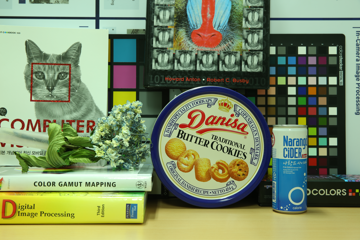
\includegraphics[width=1\textwidth]{images/resize_CC_Mean_Canon_EOS_5D_Mark3_ISO_3200_C3.png}
\end{minipage}
\begin{minipage}{0.15\textwidth}
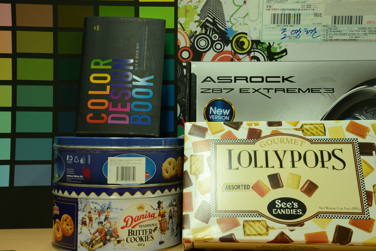
\includegraphics[width=1\textwidth]{images/resize_CC_Mean_Nikon_D600_ISO_3200_C1.png}
\end{minipage}
\begin{minipage}{0.15\textwidth}
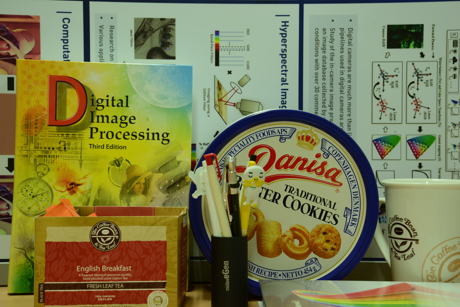
\includegraphics[width=1\textwidth]{images/resize_CC_Mean_Nikon_D800_ISO_1600_B2.png}
\end{minipage}
}\vspace{-0.14in}
\subfigure{
\begin{minipage}{0.15\textwidth}
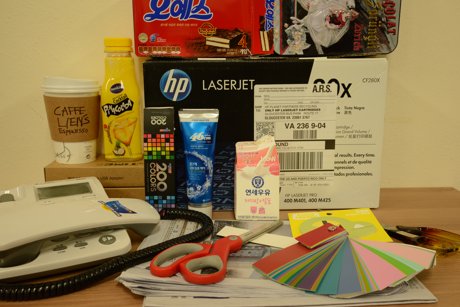
\includegraphics[width=1\textwidth]{images/resize_CC_Mean_Nikon_D800_ISO_3200_A1.png}
\end{minipage}
\begin{minipage}{0.15\textwidth}
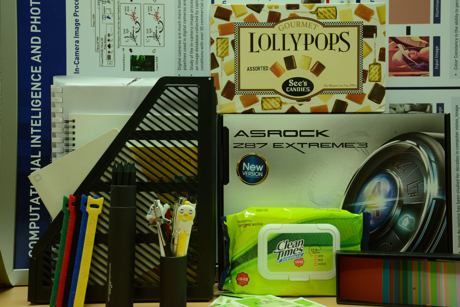
\includegraphics[width=1\textwidth]{images/resize_CC_Mean_Nikon_D800_ISO_3200_A5.png}
\end{minipage}
\begin{minipage}{0.15\textwidth}
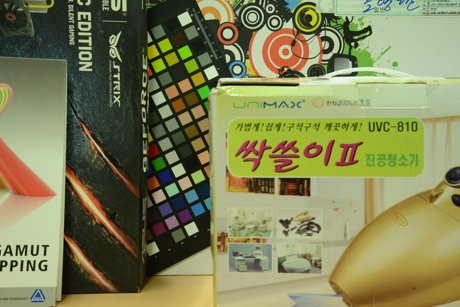
\includegraphics[width=1\textwidth]{images/resize_CC_Mean_Nikon_D800_ISO_6400_B1.png}
\end{minipage}
}
\caption{Some testing images in the dataset \cite{crosschannel2016}.}
\label{fig5}
\end{figure}

\begin{figure}[t]
\centering
\subfigure{
\begin{minipage}{0.055\textwidth}
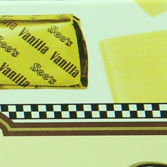
\includegraphics[width=1\textwidth]{images/resize_CC_Noisy_Canon_EOS_5D_Mark3_ISO_3200_C1_47.png}
\end{minipage}
\begin{minipage}{0.055\textwidth}
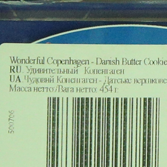
\includegraphics[width=1\textwidth]{images/resize_CC_Noisy_Canon_EOS_5D_Mark3_ISO_3200_C1_52.png}
\end{minipage}
\begin{minipage}{0.055\textwidth}
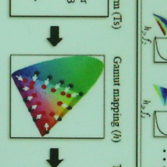
\includegraphics[width=1\textwidth]{images/resize_CC_Noisy_Canon_EOS_5D_Mark3_ISO_3200_C2_44.png}
\end{minipage}
\begin{minipage}{0.055\textwidth}
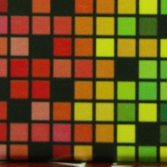
\includegraphics[width=1\textwidth]{images/resize_CC_Noisy_Canon_EOS_5D_Mark3_ISO_3200_C2_66.png}
\end{minipage}
\begin{minipage}{0.055\textwidth}
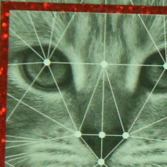
\includegraphics[width=1\textwidth]{images/resize_CC_Noisy_Canon_EOS_5D_Mark3_ISO_3200_C3_26.png}
\end{minipage}
\begin{minipage}{0.055\textwidth}

\includegraphics[width=1\textwidth]{images/resize_CC_Noisy_Canon_EOS_5D_Mark3_ISO_3200_C3_73.png}
\end{minipage}
\begin{minipage}{0.055\textwidth}
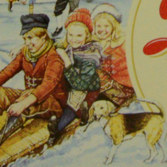
\includegraphics[width=1\textwidth]{images/resize_CC_Noisy_Nikon_D600_ISO_3200_C1_95.png}
\end{minipage}
\begin{minipage}{0.055\textwidth}
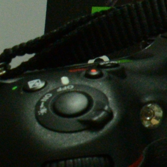
\includegraphics[width=1\textwidth]{images/resize_CC_Noisy_Nikon_D600_ISO_3200_C2_67.png}
\end{minipage}
}\vspace{-0.14in}
\subfigure{
\begin{minipage}{0.055\textwidth}
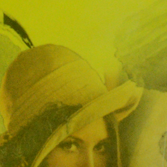
\includegraphics[width=1\textwidth]{images/resize_CC_Noisy_Nikon_D800_ISO_1600_B2_80.png}
\end{minipage}
\begin{minipage}{0.055\textwidth}
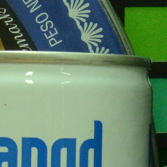
\includegraphics[width=1\textwidth]{images/resize_CC_Noisy_Nikon_D800_ISO_1600_B3_82.png}
\end{minipage}
\begin{minipage}{0.055\textwidth}
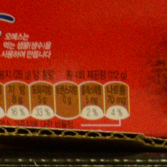
\includegraphics[width=1\textwidth]{images/resize_CC_Noisy_Nikon_D800_ISO_3200_A1_21.png}
\end{minipage}
\begin{minipage}{0.055\textwidth}
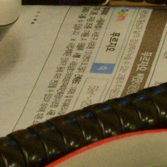
\includegraphics[width=1\textwidth]{images/resize_CC_Noisy_Nikon_D800_ISO_3200_A1_111.png}
\end{minipage}
\begin{minipage}{0.055\textwidth}
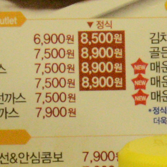
\includegraphics[width=1\textwidth]{images/resize_CC_Noisy_Nikon_D800_ISO_3200_A3_66.png}
\end{minipage}
\begin{minipage}{0.055\textwidth}
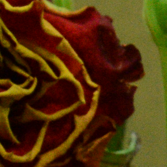
\includegraphics[width=1\textwidth]{images/resize_CC_Noisy_Nikon_D800_ISO_3200_A4_51.png}
\end{minipage}
\begin{minipage}{0.055\textwidth}
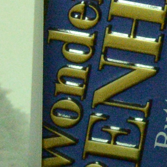
\includegraphics[width=1\textwidth]{images/resize_CC_Noisy_Nikon_D800_ISO_6400_B3_95.png}
\end{minipage}
\begin{minipage}{0.055\textwidth}
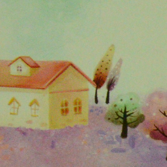
\includegraphics[width=1\textwidth]{images/resize_CC_Noisy_Nikon_D800_ISO_3200_A2_80.png}
\end{minipage}
}
\caption{Some cropped images of the dataset \cite{crosschannel2016}.}
\label{fig5}
\end{figure}

\subsection{Implementation Details}
Our proposed method contains two stages, the external prior guided internal subspace learning stage and the adaptive denoising stage. In the learning stage, there are 4 parameters: the patch size $p$, the number of patches in a PG $M$, the window size $W$ for PG searching and the number of clusters $K$. We set $p = 6$ (hence the patch size is $6\times 6 \times 3$), $M=10$, $W = 31$, $K=32$. We extracted about 3.6 million PGs from the Kodak PhotoCD Dataset, which includes 24 high quality color images, to train the external prior via PG-GMM. In the denoising stage, the paramter $\lambda = 0.002$ is used to regularize the sparse term. The $\delta$ in iterative regularization is set as $\delta = 0.09$.

\subsection{Comparison on External and Internal methods}
In this subsection, we compared the proposed external prior guided internal subspace learning model on real image denoising. The three methods are evaluated on the dataset provided in \cite{crosschannel2016}. We calculate the PSNR, SSIM \cite{ssim} and visual quality of these three methods. We also compare the speed. The PSNR and SSIM results on 60 cropped images from \cite{crosschannel2016} are listed in Table 1. The images are cropped into size of $500\times 500$ for better illustration. We also compare the three methods on visual quality in Figure \ref{fig2}. Compare the denoised images listed in Figure \ref{fig2} and Figure \ref{fig2}, we can see that the Offline method is better at edges, smooth regions while the Online method is good at complex textures. The reason is two folds. Firstly, the Offline method is learned on clean images and hence is better at representing edges, structuals, and smooth area. The online method is influenced by the noise and hence some noise cannot be removed. Secondly, the Online method is better at recovering complex area sicne they could learn adaptive dictionaries for the specific area. The Offline method cannot recover the complex area since they did not learn the similar structures from the external natural clean images.

\begin{table}\label{tab1}
\caption{Average PSNR(dB)/SSIM results of external, internal, and guided methods on 60 cropped real noisy images in \cite{crosschannel2016}.}
\label{tab1}
\begin{center}
\renewcommand\arraystretch{1}
\begin{tabular}{|c||c|c|c|c|}
\hline
 & \textbf{Noisy} &\textbf{Offline} &\textbf{Online} &\textbf{Guided}  
\\
\hline
PSNR & 34.51 & 38.19 & 38.07 & \textbf{38.55} 
\\
\hline
SSIM & 0.8718 &  0.9663   & 0.9625 & \textbf{0.9675}
\\
\hline
\end{tabular}
\end{center}
\end{table}

\begin{figure*}\label{fig2}
\centering
\subfigure{
\begin{minipage}[t]{0.195\textwidth}
\centering
\raisebox{-0.15cm}{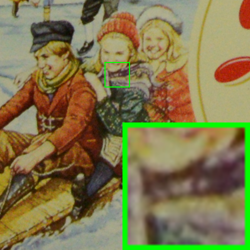
\includegraphics[width=1\textwidth]{images/resize_br_Noisy_CC_Noisy_Nikon_D600_ISO_3200_C1_95.png}}
{\footnotesize (a) Noisy Image \\ (34.66dB/0.9178)   }
\end{minipage}
\begin{minipage}[t]{0.195\textwidth}
\centering
\raisebox{-0.15cm}{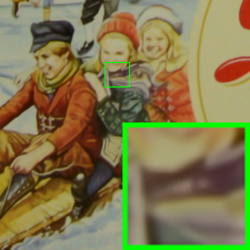
\includegraphics[width=1\textwidth]{images/resize_br_Offline_CC_Noisy_Nikon_D600_ISO_3200_C1_95.png}}
{\footnotesize (h) Offline \\ (34.97dB/0.9441) }
\end{minipage}
\begin{minipage}[t]{0.195\textwidth}
\centering
\raisebox{-0.15cm}{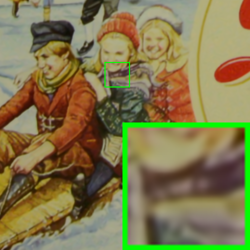
\includegraphics[width=1\textwidth]{images/resize_br_Online_CC_Noisy_Nikon_D600_ISO_3200_C1_95.png}}
{\footnotesize (i) Online \\ (36.86dB/0.9622) }
\end{minipage}
\begin{minipage}[t]{0.195\textwidth}
\centering
\raisebox{-0.15cm}{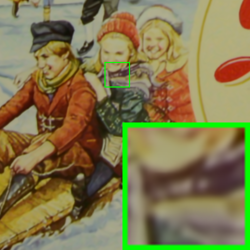
\includegraphics[width=1\textwidth]{images/resize_br_Guided_CC_Noisy_Nikon_D600_ISO_3200_C1_95.png}}
{\footnotesize (j) Guided \\ (\textbf{37.09}dB/\textbf{0.9638})}
\end{minipage}
\begin{minipage}[t]{0.195\textwidth}
\centering
\raisebox{-0.15cm}{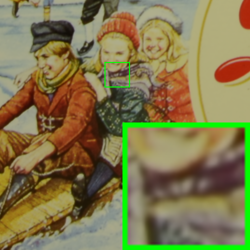
\includegraphics[width=1\textwidth]{images/resize_br_Mean_CC_Noisy_Nikon_D600_ISO_3200_C1_95.png}}
{\footnotesize (h) Mean Image }
\end{minipage}
}
\caption{Denoised images of the image "Nikon D600 ISO 3200 C1" by different methods. The images are better to be zoomed in on screen.}
\end{figure*}

\begin{figure*}\label{fig2}
\centering
\subfigure{
\begin{minipage}[t]{0.195\textwidth}
\centering
\raisebox{-0.15cm}{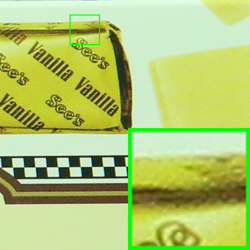
\includegraphics[width=1\textwidth]{images/resize_br_Noisy_CC_Noisy_Canon_EOS_5D_Mark3_ISO_3200_C1_47.png}}
{\footnotesize (a) Noisy Image \\ (36.15dB/0.9523)    }
\end{minipage}
\begin{minipage}[t]{0.195\textwidth}
\centering
\raisebox{-0.15cm}{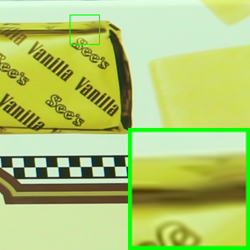
\includegraphics[width=1\textwidth]{images/resize_br_Offline_CC_Noisy_Canon_EOS_5D_Mark3_ISO_3200_C1_47.png}}
{\footnotesize (h) Offline \\ (37.12dB/0.9776) }
\end{minipage}
\begin{minipage}[t]{0.195\textwidth}
\centering
\raisebox{-0.15cm}{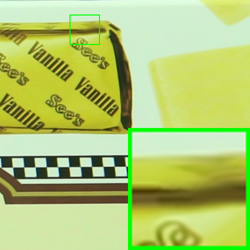
\includegraphics[width=1\textwidth]{images/resize_br_Online_CC_Noisy_Canon_EOS_5D_Mark3_ISO_3200_C1_47.png}}
{\footnotesize (i) Online \\ (35.70dB/0.9755)  }
\end{minipage}
\begin{minipage}[t]{0.195\textwidth}
\centering
\raisebox{-0.15cm}{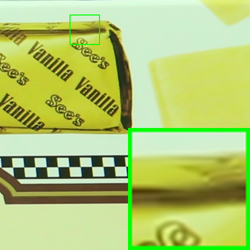
\includegraphics[width=1\textwidth]{images/resize_br_Guided_CC_Noisy_Canon_EOS_5D_Mark3_ISO_3200_C1_47.png}}
{\footnotesize (j) Guided \\ (\textbf{37.94}dB/\textbf{0.9804})}
\end{minipage}
\begin{minipage}[t]{0.195\textwidth}
\centering
\raisebox{-0.15cm}{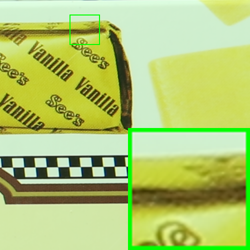
\includegraphics[width=1\textwidth]{images/resize_br_Mean_CC_Noisy_Canon_EOS_5D_Mark3_ISO_3200_C1_47.png}}
{\footnotesize (h) Mean Image }
\end{minipage}
}
\caption{Denoised images of the image "Canon EOS 5D Mark3 ISO 3200 C1" by different methods. The images are better to be zoomed in on screen.}
\end{figure*}


\subsection{Comparison With other Competing Methods}
We compare with previous state-of-the-art Gaussian noise removal methods such as BM3D \cite{bm3d}, WNNM \cite{wnnm}, MLP \cite{mlp}, CSF \cite{csf}, and the recently proposed TRD \cite{chen2015learning}. We also compare with three competing real image denoising methods such as Noise Clinic, Neat Image, and the CCNoise method proposed recently. The popular software NeatImage which is one of the best denoising software available. All these methods need noise estimation which is vary hard to perform if there is no uniform regions are available in the testing image. The NeatImage will fail to perform automatical parameters settings if there is no uniform regions. \footnote{To compare with CCNoise, we first transform the denoised images into double format.}

We the competing denoising methods from various research directions on two datasets. Both the two datasets comes from the \cite{crosschannel2016}. The first dataset contains 17 images of size over $7000\times5000$. Since this dataset contains repetitive contents across different images, we crop 60 small images of size $500\times500$ from these 17 images in \cite{crosschannel2016}.

The PSNR and SSIM resluts are listed in Table \ref{tab1}. The number in red color and blue color means the best and second best results, respectively. From the Table \ref{tab1}, we can see that the external based method can already surpass largely the previous denoising methods. The improvement on PSNR over the second best method, i.e., TRD, is 0.44dB. The 
\begin{table*}\label{tab1}
\caption{Average PSNR(dB) results of different methods on 60 cropped real noisy images captured in \cite{crosschannel2016}.}
\label{tab1}
\begin{center}
\renewcommand\arraystretch{1}
\begin{tabular}{|c||c|c|c|c|c|c|c|c|c|c|c|}
\hline
 & \textbf{Noisy} &\textbf{CBM3D}&\textbf{WNNM}&\textbf{MLP}&\textbf{CSF}&\textbf{TRD}& \textbf{NI}& \textbf{NC} &\textbf{Guided}  &\textbf{Guided2} 
\\
\hline
PSNR & 34.51 & 34.58 & 34.52 & 36.19 & 37.40 & 37.75 & 36.53 & 37.57 &  \color{blue}{38.72} & \color{red}{ 38.90}
\\
\hline
SSIM & 0.8718  & 0.8748  & 0.8743   & 0.9470 & 0.9598 &  0.9617 & 0.9241  &  0.9514  & \color{blue}{0.9694} & \color{red}{0.9702}
\\
\hline
\end{tabular}
\end{center}
\end{table*}

\begin{table*}\label{tab2}
\caption{Average PSNR(dB) results of different methods on 15 cropped real noisy images used in \cite{crosschannel2016}.}
\label{tab1}
\begin{center}
\renewcommand\arraystretch{1}
\begin{tabular}{|c||c|c|c|c|c|c|c|c|c|c|}
\hline
Camera Settings & \textbf{Noisy} &\textbf{CBM3D}&\textbf{WNNM}&\textbf{MLP}&\textbf{CSF}&\textbf{TRD}& \textbf{NI}& \textbf{NC}& \textbf{CC} &\textbf{Guided2} 
\\
\hline
\multirow{3}{*}{\small{Canon 5D Mark III}} 
& 37.00 & 37.08 & 37.09 & 33.92 & 35.68 & 36.20 & 37.68 & \color{blue}{38.76} & 38.37 & \color{red}{40.50}
\\ 
\cline{2-11} 
\multirow{3}{*}{ISO = 3200}   
& 33.88 & 33.94 & 33.93 & 33.24 & 34.03 & 34.35 & 34.87 & \color{blue}{35.69} & 35.37 & \color{red}{37.22}
\\ 
\cline{2-11}    
& 33.83 & 33.88 & 33.90 & 32.37 & 32.63 & 33.10 & 34.77 & \color{blue}{35.54} & 34.91 & \color{red}{37.13}  
\\
\hline
\multirow{3}{*}{Nikon D600} 
& 33.28 & 33.33 & 33.34 & 31.93 & 31.78 & 32.28 & 34.12 & \color{red}{35.57} & 34.98 & \color{blue}{35.34}
\\ 
\cline{2-11} 
\multirow{3}{*}{ISO = 3200}   
& 33.77 & 33.85 & 33.79 & 34.15 & 35.16 & 35.34 & 35.36 & \color{red}{36.70} & 35.95 & \color{blue}{36.69}
\\ 
\cline{2-11}    
& 34.93 & 35.02 & 34.95 & 37.89 & 39.98 & \color{blue}{40.51} & 38.68 & 39.28 & \color{red}{41.15} & 39.17
\\
\hline
\multirow{3}{*}{Nikon D800} 
& 35.47 & 35.54 & 35.57 & 33.77 & 34.84 & 35.09 & 37.34 & \color{blue}{38.01} & 37.99 & \color{red}{38.82}
\\ 
\cline{2-11} 
\multirow{3}{*}{ISO = 1600}   
& 35.71 & 35.79 & 35.77 & 35.89 & 38.42 & 38.65 & 38.57 & 39.05 & \color{blue}{40.36} & \color{red}{40.98}
\\ 
\cline{2-11}    
& 34.81 & 34.92 & 34.95 & 34.25 & 35.79 & 35.85 & 37.87 & 38.20 & \color{blue}{38.30} & \color{red}{38.90}
\\
\hline
\multirow{3}{*}{Nikon D800} 
& 33.26 & 33.34 & 33.31 & 37.42 & 38.36 & 38.56 & 36.95 & 38.07 & \color{red}{39.01} & \color{blue}{38.69}
\\ 
\cline{2-11} 
\multirow{3}{*}{ISO = 3200}   
& 32.89 & 32.95 & 32.96 & 34.88 & 35.53 & 35.76 & 35.09 & 35.72 & \color{blue}{36.75} & \color{red}{36.82}
\\ 
\cline{2-11}    
& 32.91 & 32.98 & 32.96 & 38.54 & \color{blue}{40.05} & \color{red}{40.59} & 36.91 & 36.76 & 39.06 & 38.80
\\ 
\hline
\multirow{3}{*}{Nikon D800} 
& 29.63 & 29.66 & 29.71 & 33.59 & 34.08 & \color{blue}{34.25} & 31.28 & 33.49 & \color{red}{34.61} & 33.31
\\ 
\cline{2-11} 
\multirow{3}{*}{ISO = 6400}   
& 29.97 & 30.01 & 29.98 & 31.55 & 32.13 & 32.38 & 31.38 & 32.79 & \color{red}{33.21} & \color{blue}{33.18}
\\ 
\cline{2-11}    
& 29.87 & 29.90 & 29.95 & 31.42 & 31.52 & 31.76 & 31.40 & 32.86 & \color{blue}{33.22} & \color{red}{33.35}
\\
\hline
Average PSNR & 33.41 & 33.48 & 33.48 & 34.32 & 35.33 & 35.65 & 35.49 & 36.43 & \color{blue}{36.88} & \color{red}{ 37.26}
\\
\hline
Average SSIM & 0.8483 & 0.8511 & 0.8512 & 0.9113 & 0.9250 & 0.9280 & 0.9126 & 0.9364 & \color{blue}{0.9481} & \color{red}{ 0.9505}
\\
\hline
\end{tabular}
\end{center}
\end{table*}

\begin{figure*}
\centering
\subfigure{
\begin{minipage}[t]{0.195\textwidth}
\centering
\raisebox{-0.15cm}{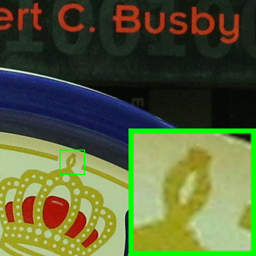
\includegraphics[width=1\textwidth]{images/resize_br_Noisy_5dmark3_iso3200_1_real.png}}
{\footnotesize (a) Noisy Image \\ (37.00dB/0.9345) }
\end{minipage}
\begin{minipage}[t]{0.195\textwidth}
\centering
\raisebox{-0.15cm}{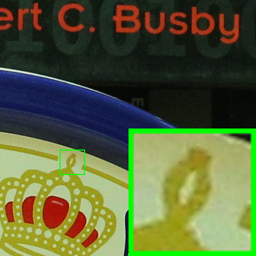
\includegraphics[width=1\textwidth]{images/resize_br_CBM3D_5dmark3_iso3200_1_real.png}}
{\footnotesize (b) CBM3D \\ (37.02dB/0.9351)}
\end{minipage}
\begin{minipage}[t]{0.195\textwidth}
\centering
\raisebox{-0.15cm}{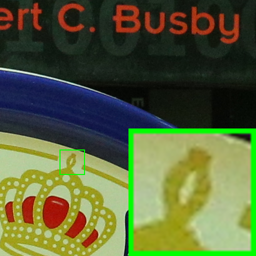
\includegraphics[width=1\textwidth]{images/resize_br_WNNM_5dmark3_iso3200_1_real.png}}
{\footnotesize (c) WNNM \\ (37.01dB/0.9347)}
\end{minipage}
\begin{minipage}[t]{0.195\textwidth}
\centering
\raisebox{-0.15cm}{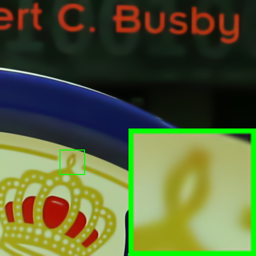
\includegraphics[width=1\textwidth]{images/resize_br_MLP_5dmark3_iso3200_1_real.png}}
{\footnotesize (d) MLP \\ (33.90dB/0.9171) }
\end{minipage}
\centering
\begin{minipage}[t]{0.195\textwidth}
\raisebox{-0.15cm}{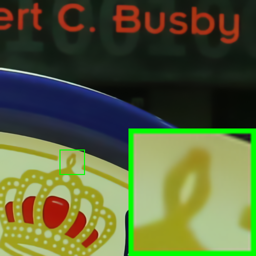
\includegraphics[width=1\textwidth]{images/resize_br_TRD_5dmark3_iso3200_1_real.png}}
{\footnotesize (e) TRD \\ (36.18dB/0.9454)   }
\end{minipage}
}
\subfigure{
\begin{minipage}[t]{0.195\textwidth}
\centering
\raisebox{-0.15cm}{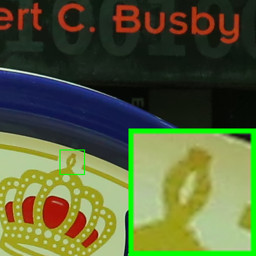
\includegraphics[width=1\textwidth]{images/resize_br_NC_5dmark3_iso3200_1_real.png}}
{\footnotesize (f) Noise Clinic \\ (38.76dB/0.9689) }
\end{minipage}
\begin{minipage}[t]{0.195\textwidth}
\centering
\raisebox{-0.15cm}{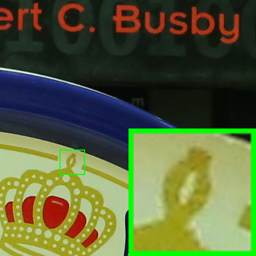
\includegraphics[width=1\textwidth]{images/resize_br_NI_5dmark3_iso3200_1_real.png}}
{\footnotesize (g) Neat Image \\ (37.68dB/0.9600) }
\end{minipage}
\begin{minipage}[t]{0.195\textwidth}
\centering
\raisebox{-0.15cm}{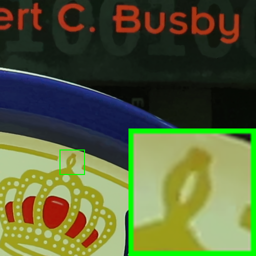
\includegraphics[width=1\textwidth]{images/resize_br_CCNoise_5dmark3_iso3200_1.png}}
{\footnotesize (h) CCNoise \\ (38.37dB/0.9678) }
\end{minipage}
\begin{minipage}[t]{0.195\textwidth}
\centering
\raisebox{-0.15cm}{\includegraphics[width=1\textwidth]{images/resize_br_Guided_5dmark3_iso3200_1_real.png}}
{\footnotesize (i) Guided \\ (\textbf{40.26}dB/\textbf{0.9800})}
\end{minipage}
\begin{minipage}[t]{0.195\textwidth}
\centering
\raisebox{-0.15cm}{\includegraphics[width=1\textwidth]{images/resize_br_Mean_5dmark3_iso3200_1_real.png}}
{\footnotesize (j) Mean Image}
\end{minipage}
}
\caption{Denoised images of the image "Canon 5D Mark 3 ISO 3200 1" by different methods. The images are better to be zoomed in on screen.}
\label{fig3}
\end{figure*}


\begin{figure*}
\centering
\subfigure{
\begin{minipage}[t]{0.244\textwidth}
\centering
\raisebox{-0.15cm}{\includegraphics[width=1\textwidth]{images/resize_br_Noisy_dog.png}}
{\footnotesize (a) Noisy Image   }
\end{minipage}
\begin{minipage}[t]{0.244\textwidth}
\centering
\raisebox{-0.15cm}{\includegraphics[width=1\textwidth]{images/resize_br_BM3D_dog.png}}
{\footnotesize (b) CBM3D}
\end{minipage}
\begin{minipage}[t]{0.244\textwidth}
\centering
\raisebox{-0.15cm}{\includegraphics[width=1\textwidth]{images/resize_br_WNNM_dog.png}}
{\footnotesize (c) WNNM    }
\end{minipage}
\begin{minipage}[t]{0.244\textwidth}
\centering
\raisebox{-0.15cm}{\includegraphics[width=1\textwidth]{images/resize_br_MLP_dog.png}}
{\footnotesize (d) MLP }
\end{minipage}
}
\subfigure{
\begin{minipage}[t]{0.244\textwidth}
\centering
\raisebox{-0.15cm}{\includegraphics[width=1\textwidth]{images/resize_br_TRD_dog.png}}
{\footnotesize (e) TRD }
\end{minipage}
\begin{minipage}[t]{0.244\textwidth}
\centering
\raisebox{-0.15cm}{\includegraphics[width=1\textwidth]{images/resize_br_NC_dog.png}}
{\footnotesize (f) Noise Clinic   }
\end{minipage}
\begin{minipage}[t]{0.244\textwidth}
\centering
\raisebox{-0.15cm}{\includegraphics[width=1\textwidth]{images/resize_br_NI_dog.png}}
{\footnotesize (g) Neat Image    }
\end{minipage}
\begin{minipage}[t]{0.244\textwidth}
\centering
\raisebox{-0.15cm}{\includegraphics[width=1\textwidth]{images/resize_br_Guided_dog.png}}
{\footnotesize (h) Guided  }
\end{minipage}
}
\caption{Denoised images of the image "$5dmark3 iso3200 3$" by different methods. The images are better to be zoomed in on screen.}
\label{fig4}
\end{figure*}

\subsection{Discussion on Parameter $\lambda$}
The proposed method only has a key parameter, namely the regularization paramters $\lambda$. To demonstrate that the proposed method is robust to the variance of $\lambda$, we vary the parameter $\lambda$ across a wide range and obtain the PSNR and SSIM results as a function of the parameter $\lambda$. The results is shown in Figure \ref{fig10}, from which we can see that the proposed method can achieve a PSNR (SSIM) over 38.5dB (0.9660) when $\lambda$ varies from $0.0015$ to $0.0025$. This shows that the proposed method is indeed robust to the chosen of the paramter $\lambda$.
\begin{figure}
\includegraphics[width=1\linewidth]{images/param.png}
\caption{The PSNR/SSIM results as a function of the parameter $\lambda$.}
\label{fig10}
\end{figure}

\section{Conclusion and Future Work}

In the future, we will evaluate the proposed method on other conputer vision tasks such as single image super-resolution, photo-sketch synthesis, and cross-domain image recognition. Our proposed method can be improved if we use better training images, fine tune the parameters via cross-validation. We believe that our framework can be useful not just for real image denoising, but for image super-resolution, image cross-style synthesis, and recognition tasks. This will be our line of future work.

{\small
\bibliographystyle{unsrt}
\bibliography{egbib}
}

\end{document}
